\begin{frame}
\begin{figure}
\centering
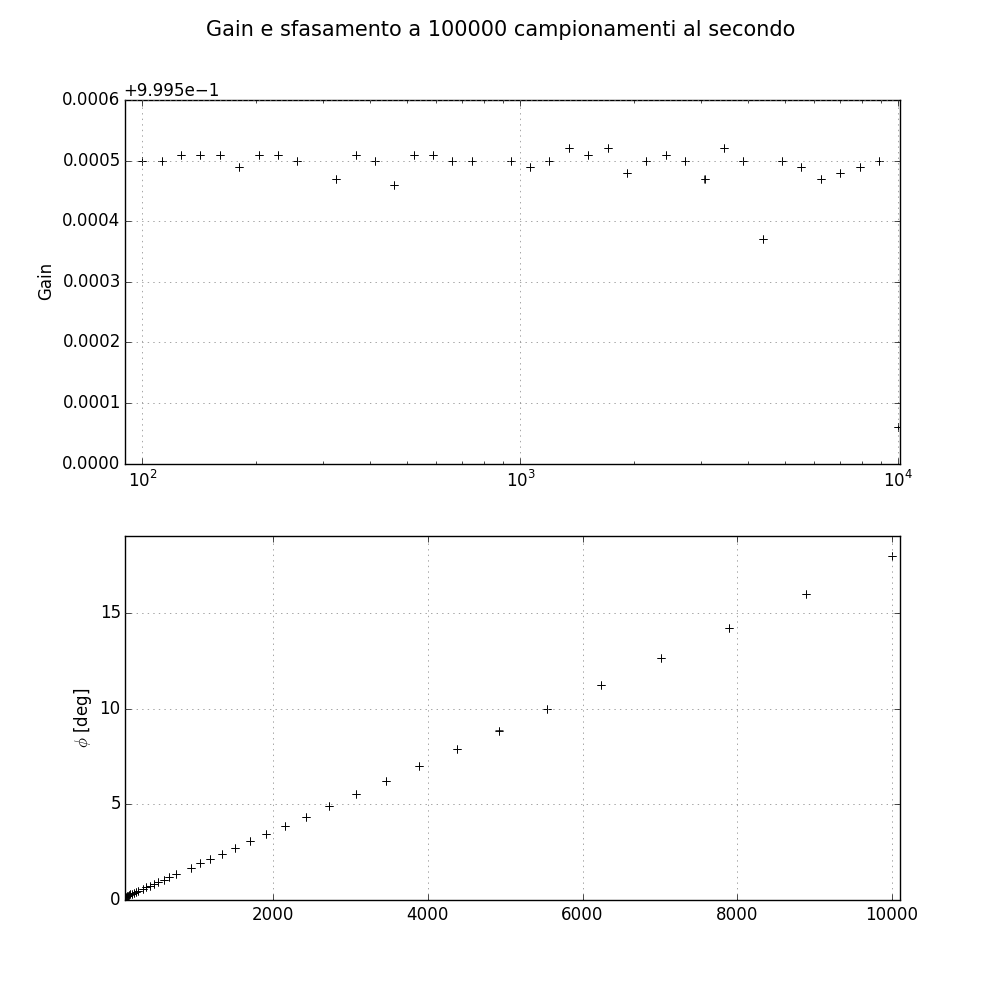
\includegraphics[width=0.9\linewidth]{./subplots_errors_amplitude100000}
\caption{Gain e sfasamento con 100000 campioni al secondo}
\label{fig:sfasamento100000}
\end{figure}
\end{frame}

\begin{frame}
\begin{figure}
\centering
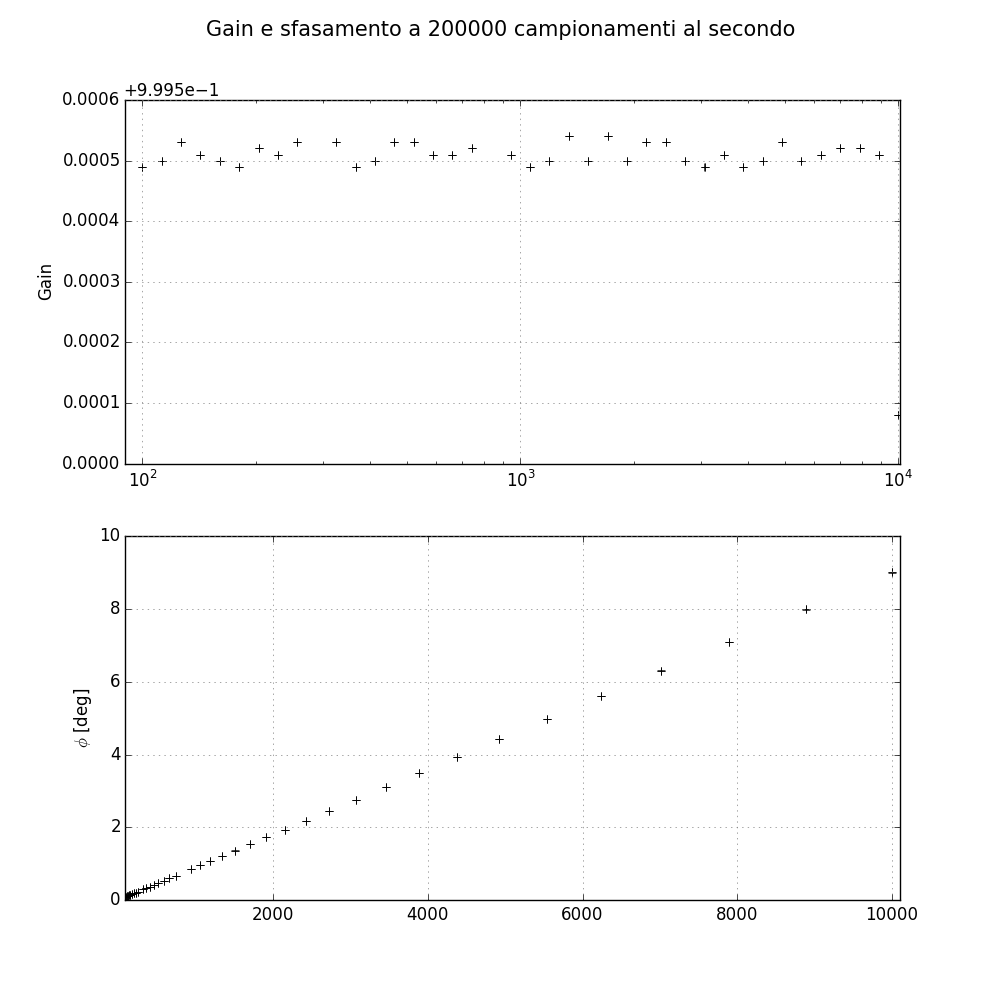
\includegraphics[width=0.9\linewidth]{./subplots_errors_amplitude200000}
\caption{Gain e sfasamento con 200000 campioni al secondo}
\label{fig:sfasamento200000}
\end{figure}
\end{frame}

\begin{frame}
\begin{figure}
\centering
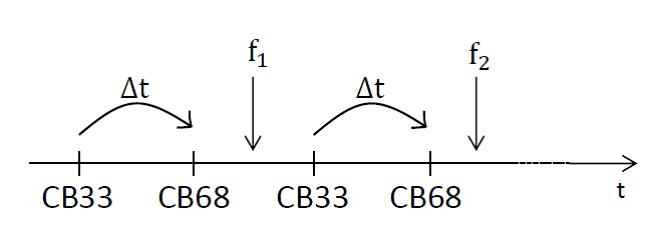
\includegraphics[width=0.9\linewidth]{immagine}
\caption{Schema processo di acquisizione}
\label{fig:schema}
\end{figure}
\begin{itemize}
\item $\Delta \varphi = \Delta tf$, $\Delta t = \frac{\alpha}{f_c}$, $\alpha = 179.97 \pm 0.11$
\item Algoritmo correttivo:\\
\begin{equation}
\varphi ' = \varphi - \alpha \frac{f}{f_c}
\end{equation}
\end{itemize}
\end{frame}

\begin{frame}
\begin{figure}
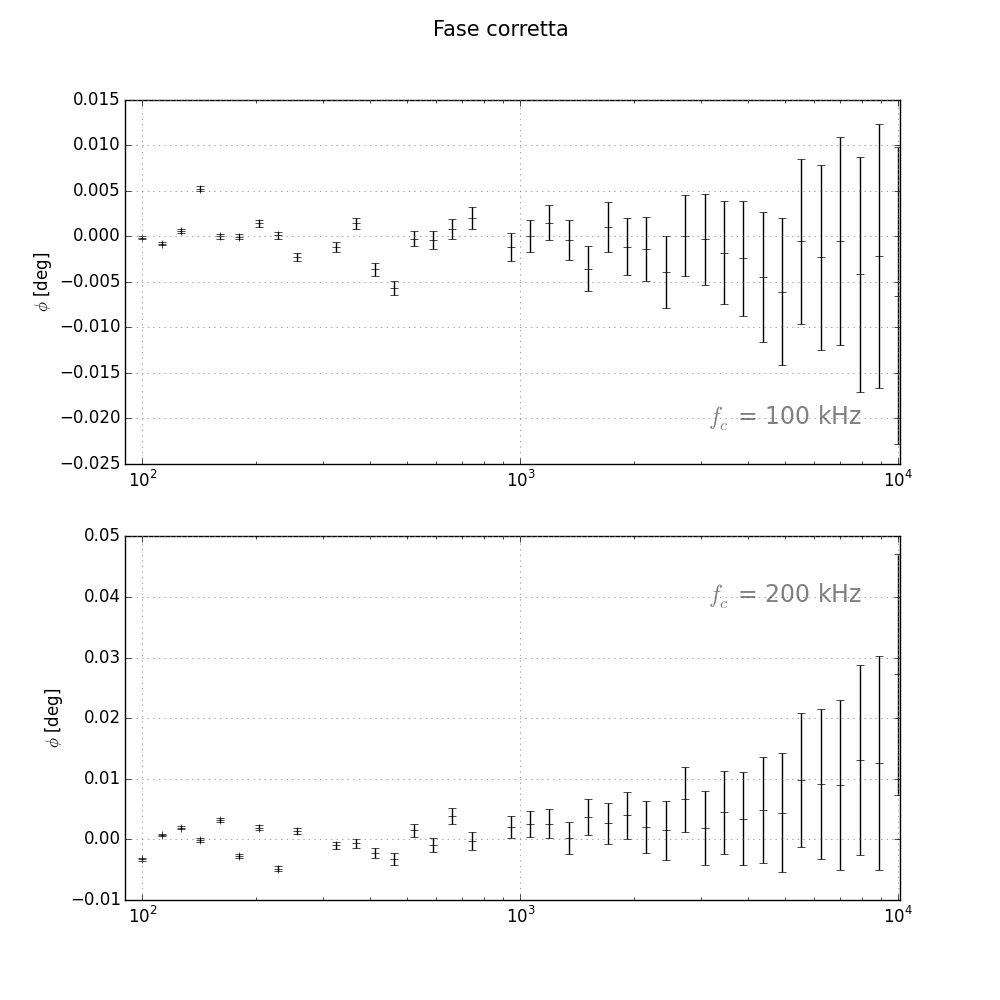
\includegraphics[width=0.9\linewidth]{subplots_errors}
\caption{Sfasamenti con algoritmo correttivo}
\label{fig:sfasacorret}
\end{figure}
\end{frame}